% text copied from early NSF grant draft (unused in final grant)

Memory researchers, like cognitive neuropsychologists in many domains, have
historically taken a ``less is more'' approach. They follow the logic that,
given a memory topic of interest (e.g.\ memory for real-world autobiographical
events), we can ask: what is the simplest experimental paradigm that we might
reasonably expect to involve a shared or analogous set of behavioral tendencies
and brain structures? There are many benefits to taking a simplified approach
to studying complex cognitive phenomena. By composing a set of experimental
circumstances where every aspect of the stimuli and timing is carefully
controlled by the experimentalist, and where the behaviors a participant can
exhibit are highly constrained, it becomes possible to systematically link
specific experimental observations to their corresponding neural and behavioral
mechanisms~\citep{OReiMuna00}. However, there is also a major cost to
simplifying: tightly controlled experiences designed in the lab can often only
provide indirect insights into the real-world analogs of those experiences.
This has led to a major hole in the memory theory literature. On the one hand,
the most well-developed theories of human memory have been informed by a long
history of tightly controlled (but simplified relative to the real-world)
experiments~\citep[e.g.\ list-learning, priming, reaction times; ][]{Kaha12}.
On the other hand, studies of real-world classroom learning have largely
avoided drawing direct links with those theories, instead focusing on questions
about applied topics such as creating effective assessment tools, increasing
student engagement and motivation, and understanding what makes an effective
teacher~\citep{Seid07}.

The general approach we take in our project is to use prior experimental and
theoretical work on list learning as a foundation for optimizing STEM learning.
Specifically, \textbf{Module 1 is centered around developing approaches for
improving participants' memories for lists of words-- a simple and well-studied
task expected to involve neural mechanisms similar to those underlying STEM
learning}. To foreshadow our proposal, \textbf{in Module 2, we have designed a
set of analogous experiments and analyses that adapt the approach in Module 1
to a more naturalistic learning setting (learning from online STEM training
videos)}. By mirroring our approaches in Modules 1 and 2, we hope to be able to
draw parallels between the two sets of experiments and findings. Finally,
\textbf{in Module 3, we plan to replicate the EEG experiments in Modules 1 and
2 using a low-cost EEG system that our team developed. We will also develop
(and document) an open-source toolkit for sharing our software (and data). In
this way, Module 3 will serve to help bring our work into real-world
classrooms, and to real-world students}.

\subsection*{Context and the structure of memory} 

Remembering words on a studied list requires distinguishing the current list
from the rest of one's experience. To model this fundamental memory capability,
cognitive scientists have posited the existence of a special representation,
called \emph{context}, that is associated with each list. According to early
theories~\citep[e.g.][]{Este55a,AndeBowe72} context representations are
composed of many features which fluctuate from moment to moment, slowly
drifting through a multidimensional feature space. During recall, this
representation forms part of the retrieval cue, enabling us to distinguish list
items from non-list items. Understanding the role of context in memory
processes is particularly important in self-cued memory tasks, such as
\textit{free recall}, where the retrieval cue is ``context'' itself. In free
recall, participants study lists of items and are instructed to recall the
items in any order they choose.

\begin{wrapfigure}[10]{r}{1.3in}
  \begin{center}
    \vspace{-33pt}
    \includegraphics[width=1.1in]{figs/fingerprint_schematic.pdf}
  \end{center}
  \vspace{-18pt}
  \caption{\footnotesize \textbf{Memory fingerprint.}  Reflects a participant's tendency to cluster recalls according to each stimulus feature dimension.}
  \label{fig:fingerprint}
\end{wrapfigure}

Over the past half-century, context-based models have enjoyed impressive
success at explaining many stereotyped behaviors observed during free recall
and other list-learning tasks \citep[e.g.][]{Este55a, RaaiShif80, GlenEtal83,
HowaKaha02a, SiroEtal05, KimbEtal07, PolyKaha08, PolyEtalTulv, SedeEtal08,
PolyEtal09, ShanHowa12}. These phenomena include the well-known recency and
primacy effects (superior recall of items from the end and, to a lesser extent,
from the beginning of the study list), as well as semantic and temporal
clustering effects \citep[for review see][]{KahaEtal08}. The contiguity effect
is an example of temporal clustering, which is perhaps the dominant form of
organization in free recall. This effect can be seen in the tendency for people
to successively recall items that occupied neighboring positions in the study
list. For example, if a list contained the sub-sequence \textsc{``absence
hollow pupil''} and the participant recalls the word \textsc{``hollow''}, it is
far more likely that the next response will be either \textsc{``pupil''} or
\textsc{``absence''} than some other list item~\citep{Kaha96}. In addition,
there is a strong forward bias in the contiguity effect: subjects make forward
transitions (i.e., \textsc{``hollow''} followed by \textsc{``pupil''}) about
twice as often as they make backward transitions, despite an overall tendency
to begin recall at the end of the list. There are also striking effects of
semantic clustering \citep{RomnEtal93, Bous53, BousEtal54, JenkRuss52,
MannKaha12}, whereby the recall of a given item is more likely to be followed
by recall of a similar or related item than a dissimilar or unrelated one.

In general, people organize memories for words along a wide variety of stimulus
dimensions. As captured by models like the \textit{Context Maintenance and
Retrieval Model}~\citep{PolyEtal09}, the stimulus features associated with each
word (e.g.\ the word's meaning, font size, font color, location on the screen,
size of the object the word represents, etc.) are incorporated into the
participant's mental context representation~\citep[also see][]{SmitVela01,
MannEtal15}. During a memory test, any of these features may serve as a memory
cue, which in turn leads the participant to recall in succession words that
share stimulus features. We refer to a participant's particular tendency to
organize their recalls according to each stimulus dimension as their
\textit{memory fingerprint} (Fig.~\ref{fig:fingerprint}). Formally, the memory
fingerprint is a vector whose elements range between 0 and 1, where each
element of the memory fingerprint reflects a stimulus feature. A value close to
1 indicates that the participant nearly always orders their recalls according
to the given stimulus dimension. A value close to 0 indicates that the
participant almost \textit{never} orders their recalls according to the given
stimulus dimension; a value close to 0.5 indicates that the participant's
recalls are random with respect to that stimulus dimension. In Experiment 1 we
propose a free recall variant where each stimulus has many well-defined and
quantifiable features, enabling us to track how the ways people organize their
memories (i.e., their memory fingerprints) change over time. In Experiment 2 we
use a behavior-driven approach to manipulate these processes, and in Experiment
3 we use electroencephalographic (EEG) data to manipulate these processes. In
this way, Experiment 1 is focused on elucidating the dynamics of this very
specific form of learning, and Experiments 2 and 3 are focused on manipulating
the learning process, with the goal of improving (or diminishing) learning
efficiency.


\subsection*{The feature-rich free recall paradigm}

\begin{wrapfigure}[10]{r}{1.4in} \vspace{-57pt} \begin{center}
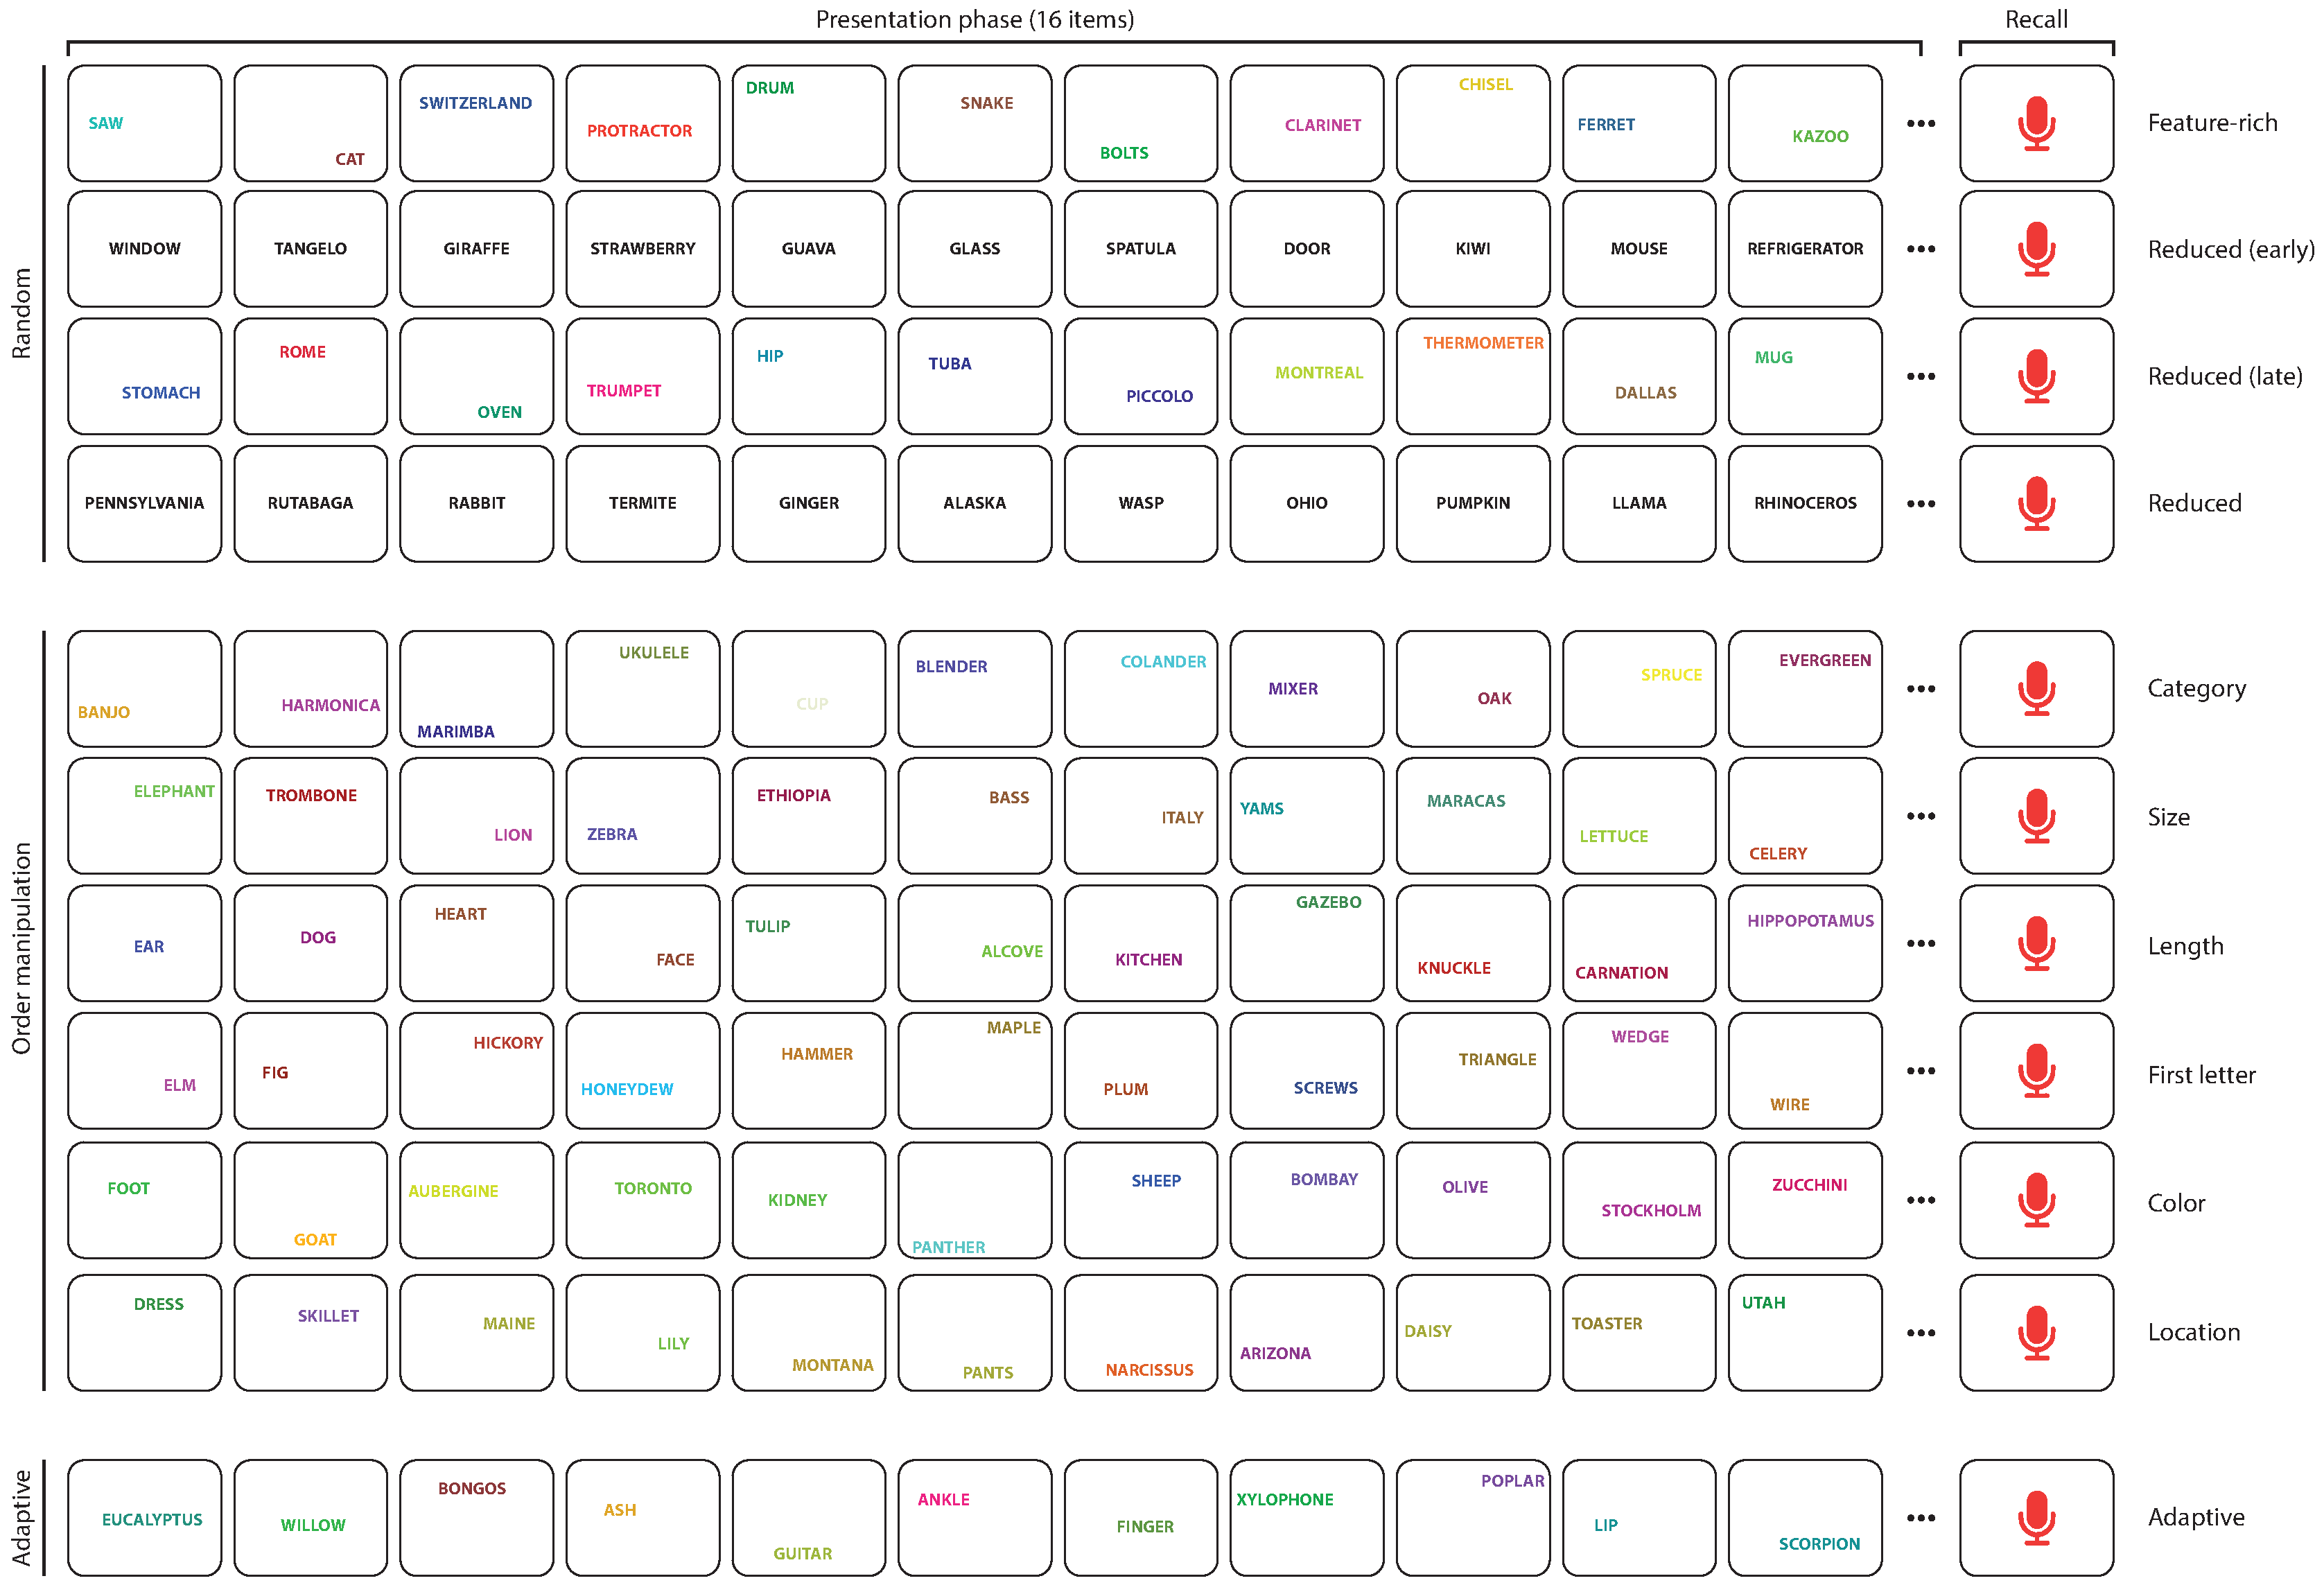
\includegraphics[width=1.2in]{figs/FRFR} \end{center} \vspace{-16pt}
\caption{\footnotesize \textbf{Feature-rich free recall.} After studying lists
comprised of words that vary along several feature dimensions, participants
verbally recall words in any order (microphone icon).} \label{fig:exp1}
\end{wrapfigure}

Each of our Module 1 experiments is based on a variant of the classic free
recall paradigm that we term \textit{feature-rich free recall}. In feature-rich
free recall, participants study 16 lists, each comprised of 16 words that vary
along a number of stimulus dimensions: semantic category, object size, text
color, text location, word length, and starting letter (Fig.~\ref{fig:exp1}).
Each list contains four words from each of four different semantic categories;
all other stimulus features are randomized. Each word is presented for 2
seconds, followed by a 2 second pause (blank screen). After studying each list,
the participant has 60 seconds to recall as many words as they can from that
list, in any order they choose. Because each individual word is associated with
several well-defined (and quantifiable) features, and because each list
incorporates a diverse mix of feature values along each dimension, this allows
us to evaluate participants' memory fingerprints in rich detail.

Our experimental paradigm incorporates the Google Cloud Speech API
speech-to-text engine to automatically transcribe participants' verbal recalls
into text. This allows recalls to be transcribed in real time-- a
distinguishing feature of the experiment that is critical for using
participants' recalls of prior lists to adapt the presentation orders of future
lists, as in Experiments 2 and 3. (In typical verbal recall experiments the
audio data must be parsed manually, precluding this sort of design.) We
recently published a study verifying that the computer-generated recall
transcripts are sufficiently similar to human-generated transcripts to yield
reliable data~\citep{ZimaEtal18}. \subsection*{Experiment 1: tracking the
dynamics of memory organization over successive learning trials} % maybe this
could benefit from reframing wrt to the variance idea? Large portions of the
memory theory and education literatures have focused on identifying learners'
unique learning styles. In the memory theory literature~\citep{SmitVela01,
Kaha12, HealKaha14a, MannEtal15}, the focus has been on identifying behavioral
signatures of how memories are organized (i.e., in the language of this
proposal, identifying memory fingerprints). In the education literature, the
focus has been been on asking whether catering lessons to an individual's
unique learning style can help them to learn more
efficiently~\citep{PashEtal08}. Each of these literatures effectively treats
people's learning styles as a fixed point. \textbf{In other words, the
assumption underlying the majority of these studies is that each individual has
their own unique learning style, and that learning style remains roughly
consistent over time. Experiment 1 is designed to explicitly test this
assumption using the feature-rich free recall paradigm (Fig.~\ref{fig:exp1}).}
Importantly, we will collect data from two populations: (a) members of the
Dartmouth and surrounding community, with the experiment running in a tightly
controlled laboratory setting, and (b) Mechanical Turk workers, via the
Internet. Taken together, we hope that these two populations of participants
will allow us to generalize our findings to a diverse set of learners.

\paragraph{Design and procedure.}

We will use the feature-rich free recall paradigm (Fig.~\ref{fig:exp1}) to
study how people's memory fingerprints are influenced by presentation order.
The experiment will be divided into six manipulation conditions (one for each
stimulus feature); in each of these manipulation conditions the words from the
first 8 lists participants study will be sorted according to one of the
stimulus dimensions. For example, in the ``color'' condition, words from the
first 8 lists will be sorted by font color; in the ``starting letter''
condition, words from the first 8 lists will be sorted alphabetically; etc. The
second 8 lists will be presented in a random order in every condition. As
described below, we will assess how participants' memories are affected by
these order manipulations, both for their memories of words on first 8 lists
where the manipulations are applied, as well as on the second 8 lists.
Participants' behaviors will be compared to a seventh (control) condition,
where the presentation order is randomized for all 16 lists.

We carried out a power analysis (power: 0.8, Type 1 error rate: 0.05) using our
prior work to estimate the relevant parameters~\citep{MannEtal11, MannEtal12}.
The analysis indicated that we will require 30 in-laboratory participants in
each of the six manipulation conditions to achieve sufficient power. Because
all of our findings will be compared relative to the random control condition,
we plan to run 60 in-laboratory participants in that condition. Prior work
suggests that Mechanical Turk data is more variable than data collected in the
laboratory~\citep{CrumEtal13}, so in each condition we plan to collect data
from twice as many Mechanical Turk workers as in-laboratory participants. In
all, across the 7 experimental conditions, we plan to run 720 participants in
Experiment 1 (240 in the lab and 480 online through Mechanical Turk).

\paragraph{Key analyses.}

Experiment 1 is motivated by two fundamental questions about the dynamics of
memory organization and recall. \textbf{First, we want to understand how memory
fingerprints vary across people and over time.} For example, are people's
memory fingerprints generally stable across lists? Or, what are the
similarities and differences across people (in how people organize their
memories, and how their memory fingerprints change over time)? Are those
individual differences predictive of memory performance? \textbf{Second, we
want to understand how people's memory fingerprints can be manipulated.}
Specifically, if lists are sorted according to a particular feature (e.g. the
words' semantic categories), how does that influence people's tendencies to
cluster their recalls of those words with respect to that feature? And which of
those tendencies persist during recalls of later (randomly ordered) lists? For
example, if we organize early lists alphabetically, are participants more
likely recall the words from those lists alphabetically as well? More
generally, might there be some way of influencing how people organize their
memories, even after the influencing cue is no longer present?

% figures: pilot data displaying random-condition fingerprints, relationship
between fingerprint variance and memory \begin{wrapfigure}[10]{R}{4.0in}
\vspace{-52pt} \begin{center}
\includegraphics[width=4.0in]{figs/random_pilot.pdf} \end{center}
\vspace{-18pt} \caption{\footnotesize \textbf{Preliminary data for feature-rich
free recall.} \textbf{a.} Clustering scores along each feature dimensions (i.e.
memory fingerprints). Each dot represents the average clustering score along
one dimension, for one participant. \textbf{b.} Across-subject correlation
between fingerprint variability and memory performance. \textbf{c.}
Across-condition correlation between fingerprint variability and memory
performance.} \label{fig:random_pilot} \end{wrapfigure}

\paragraph{Experiment 1 preliminary data.}

We ran a preliminary study ($n = 172$) to measure participants' memory
fingerprints under the in-laboratory conditions outlined in Experiment 1. Using
data from the control condition (where all lists were ordered randomly; $n =
45$), we computed the distribution of average memory fingerprints (across
lists) from each participant (Fig.~\ref{fig:random_pilot}a). The degree to
which participants organize their memories with respect to each feature varies
substantially across people (e.g.\ there is a wide spread of values covered
across participants within each feature dimension). In addition, some features
are more likely to be leveraged in people's memories than others. For example,
participants are more likely to organize their recalls by category, size, and
temporal proximity than by font color or word length. We also examined how
stable participants' memory fingerprints were across lists. We found that
participants whose memory fingerprints were more stable across lists (i.e.,
lower variance) remembered more words (Fig.~\ref{fig:random_pilot}b). We also
examined the manipulation conditions, where the first 8 lists participants
studied were sorted according to one feature (category: $n=21$, color: $n=20$,
screen location: $n=21$, first letter: $n=20$, word length: $n=23$, size:
$n=22$). Relative to randomly sorted lists, sorting by some features increased
the average memory fingerprint variability and sorting by other features
decreased the average memory fingerprint variability. (We used a
permutation-based procedure to compute the variability, which controlled for
the distributions of feature values of the words participants remembered.) We
found that participants remembered more words in the conditions where the
presentation orders led to lower fingerprint variability
(Fig.~\ref{fig:random_pilot}c). Taken together, these preliminary data suggest
that participants who naturally exhibit more stable fingerprints remember more
words, and fingerprint stability may be influenced by the order in which words
are presented. In turn, sorting the word presentations along different
dimensions can enhance (or diminish) memory performance according to whether
fingerprint variability is increased or decreased, respectively.

\subsection*{Experiment 2: adaptive list learning using (behavioral) memory fingerprints}
\begin{wrapfigure}[9]{R}{1.6in}
  \vspace{-25pt}
  \begin{center}
    \includegraphics[width=1.5in]{figs/adaptive_fr_flowchart.pdf}
  \end{center}
\vspace{-20pt}
  \caption{\footnotesize \textbf{AdaptiveFR.}  The average memory fingerprint is updated after recalling each list, and is used to determine the presentation order of the next list.}
  \label{fig:adaptiveFR_flowchart}
\end{wrapfigure}

Our pilot data from Experiment 1 suggest that the order in which words are
studied affects how they are later recalled. Further, certain orderings can
lead to lower memory fingerprint variability, which in turn leads (on average)
to better memory for the studied words. Whereas Experiment 1 explores the
memory effects of pre-defined order manipulations, in Experiment 2 we propose
to adapt the presentation order of future lists, using behavior measured on
previous lists. \textbf{Our overarching goal is to explore whether memory
models that are custom-fit to individual participants may be exploited (through
presentation order manipulations) to enhance or diminish memory performance.}

\begin{wrapfigure}[24]{R}{2in}
  \vspace{-25pt}
  \begin{center}
    \includegraphics[width=2in]{figs/adaptive_pilot}
  \end{center}
\vspace{-20pt}
  \caption{\footnotesize \textbf{AdaptiveFR pilot data. a.} Fingerprint variability decreases when lists are sorted according to the average memory fingerprints from prior lists (stabilize condition).  \textbf{b.}  Stabilizing memory fingerprints improves recall specifically for middle-of-the-list words.}
  \label{fig:adaptive_pilot}
\end{wrapfigure}

\paragraph{Design and procedure.} We will use a modified version of the feature-rich free recall paradigm designed to enhance or diminish participants' memory performance by adaptively adjusting the presentation order of future lists using recall data from previous lists (\textit{AdaptiveFR}; Fig.~\ref{fig:adaptiveFR_flowchart}).  As in Experiment 1, participants in Experiment 2 will study 16 lists.  The first 4 lists will be sorted randomly; these are used to compute the participants' individualized memory fingerprints.  Each of the remaining 12 lists (grouped into three blocks of 4 lists) will be sorted according to one of three algorithms (every participant will study and recall lists sorted using all three algorithms, but in a block-randomized order).   In the \textit{stabilize} condition, the list words will be sorted into an order that matches the participant's average memory fingerprint from all prior lists.  For example, if the memory fingerprint indicates a strong tendency to cluster recalls by category, words from the same category will tend to appear at adjacent study positions on ``stabilize'' lists.  To the extent to which the presentation order influences recall order, the stabilize condition should reduce variability in participants' memory fingerprints (by influencing future memory fingerprints to match the current average fingerprint). In the \textit{destabilize} condition, words will be sorted in an attempt to maximize the fingerprint variability.  Specifically, we will generate 10,000 random permutations of each to-be-presented list, compute a memory fingerprint for each (treating each permutation as if it were a recall sequence), and select the permutation whose fingerprint is most different (in terms of Mahalanobis distance) from the average fingerprint from prior lists.  Finally, in the \textit{random} condition, words will be shuffled randomly; this condition will be used as a baseline for the others.  We also plan to run series of analogous yoked control conditions in a second set of participants, whereby memory fingerprints based on \textit{other} participants' recalls are used to sort future lists.



We carried out a power analysis (power: 0.8, Type 1 error rate: 0.05) using our
pilot data as a guide (Fig.~\ref{fig:adaptive_pilot}). The analysis indicates
that we will require at least 33 in-laboratory participants to achieve
sufficient power, which we plan to round up to 40 participants. Similarly
(following our logic from Experiment 1) we plan to run 80 Mechanical Turk
workers in the online version of Experiment 2. We will also duplicate the
experiment using yoked controls, for a total of 80 in-laboratory and 160
Mechanical Turk participants.



\paragraph{Key analyses.}  The primary questions driving Experiment 2 concern how list order manipulations can influence memory.  \textbf{First, we want to understand whether we can adaptively enhance or diminish memory performance by increasing or decreasing the stability of people's memory fingerprints.}  Essentially, Experiment 2 is intended to serve as a strong test of our hypothesized causal link between the stability of people's memory fingerprints and their memory performance.  We will test whether our experimental manipulations can indeed influence fingerprint stability, and if so, whether those manipulations also impact memory performance.  \textbf{Second, we want to understand the extent to which these person-specific reordering manipulations are beneficial, relative to population-driven reordering manipulations.}  For example, if we customize the word presentation orders based on an individual's data, do we see stronger effects on their performance than if we had instead customized the lists based on the average data from other participants?

\paragraph{Pilot data.}  We ran a pilot study ($n = 12$) to test the feasibility of our approach.  We found that when word lists were sorted to be consistent with a participant's memory fingerprint (the stabilize condition), this led to lower fingerprint variability ($t(11) = 1.94, p = 0.06$; Fig.~\ref{fig:adaptive_pilot}a) and enhanced memory (Fig.~\ref{fig:adaptive_pilot}b).  Notably, this memory enhancement was specific to words from the middle of the list (positions 8--12; $t(11)=3.18, p=0.008$). This provides preliminary evidence that manipulations that increase the stability of participants' recall tendencies also improve memory.



\subsection*{Experiment 3: adaptive list learning using (neural) memory fingerprints}

The above experiments leverage participants' \textit{behaviors} (i.e., the
sequences of recalls they make) to optimize learning by changing the order in
which subsequent lists are presented. In Experiment 3, we seek to optimize
learning using \textit{neural} (EEG) data. \textbf{Our prior work shows that
the neural patterns recorded while participants study a list of words may be
used to predict their individual tendencies to cluster their recalls according
to presentation order (temporal clustering; Fig.~\ref{fig:clust}a) or word
meaning (semantic clustering; Fig.~\ref{fig:clust}b).}



% Logically, there are two sets of factors that can contribute to recall order.  The first set of factors are processes that occur at the time information is encoded.  The results summarized in Figure~\ref{fig:clust} show that some information about the order in which words on a studied list will later be recalled may be predicted from neural recordings taken at the time of the words are studied (encoded).  The second set of factors that can contribute to recall order occur at retrieval.  Any additional processes or stimuli that occur as the participant recalls the words could conceivably affect recall order.  For example, a sudden pang of hunger or boredom that happens to occur during the recall phase of the experiment might lead the participant to recall other words associated with those new thoughts.  The neural patterns recorded as the participant studies a list of words cannot be used to recover order effects driven by retrieval-specific processes.


\begin{wrapfigure}[12]{R}{2.5in}
\vspace{-32pt}
  \begin{center}
    \includegraphics[width=2.5in]{figs/neural_predictors_of_clustering.pdf}
  \end{center}
\vspace{-19pt}
  \caption{\footnotesize \textbf{Pilot data: neural signatures of memory fingerprints.}  Electrophysiological data recorded during study may be used to predict the degree to which a participant will later (\textbf{a.}) temporally cluster their recalls; panel adapted from~\citep{MannEtal11} or (\textbf{b.}) semantically clustering their recalls; panel adapted from~\citep{MannEtal12}.}
  \label{fig:clust}
\end{wrapfigure}

In Experiment 3, we ask whether these prior findings extend to additional dimensions of the memory fingerprint (i.e., how participants order their recalls of words).  Following from our prior work, we will record EEG activity (wavelet-derived mean spectral power in 50 log-spaced frequency bands, from each electrode) as each word is studied~\citep{MannEtal11, MannEtal12}.  We will also examine patterns of cross-frequency coupling and other dynamic connectivity patterns~\citep{MannEtal14b}.  We will then identify a neural predictor for each dimension of the memory fingerprint-- i.e., one neurally derived predictor each of how likely the word being studied will follow a word matching the same semantic category, or with a similar color, location, starting letter, etc.  Specifically, to obtain each predictor (e.g.\ of clustering recalls by color), we will consider the set of correctly recalled words (excluding the first).  For each recall in turn, we will ask: considering the dimension of interest (e.g.\ font color), how similar is each not-yet-recalled word to the previous recall?  We will use the distribution of similarity values to tag each correct recall with a percentile rank.  Regressing the neural activity recorded just before each word was studied against these percentile ranks will yield a neural predictor (classifier) of clustering by the given memory fingerprint dimension.  (This process must be repeated for each memory fingerprint dimension in turn.)  These neural predictors will be updated after each recall interval, and will be used during the study period of the next list to select each word to be presented next according to the ongoing neural recordings (Fig.~\ref{fig:adaptiveFR_eeg_order}).

\begin{wrapfigure}[11]{R}{1.7in}
\vspace{-46pt}
  \begin{center}
    \includegraphics[width=1.5in]{figs/adaptive_fr_EEG_flowchart.pdf}
  \end{center}
\vspace{-23pt}
  \caption{\footnotesize \textbf{AdaptiveFR with EEG.}  EEG recordings during study are used to update the memory fingerprint classifier after each batch of recalls.  The classifier is used to adapt the presentation order on a word-by-word basis when the next list is studied.}
  \label{fig:adaptiveFR_eeg_order}
\end{wrapfigure}

\paragraph{Design and procedure.} 

The experiment and parameters will be analogous to Experiment 2, except that we
will use EEG data recorded as participants are studying the words (rather than
behavioral data from participants' recalls) to estimate their memory
fingerprints. We plan to record the EEG data using an ActiChamp 160-electrode
system (with a photosensor-based electrode mapping system, to allow us to
perform source-localization analyses). Participants will study a total of 16
lists of 16 words each; we will adaptively adjust the presentation orders of
each list as described next.

The first four lists will always be sorted randomly. We will use EEG recordings
as participants study these lists to train classifiers to detect the neural
signatures of clustering along each memory fingerprint dimension. Note that,
whereas in Experiment 2 the presentation order of the full list is determined
before the first word is presented, in Experiment 3 we will be adaptively
adjusting the presentation order on a word-by-word basis using classifiers
applied to the ongoing EEG recordings. In other words, we will use the EEG
activity recorded during the inter-stimulus interval to predict how the next
word will be organized in memory. Then, using the just-presented word as a
reference, we will select a word that is either \textit{consistent},
\textit{inconsistent}, or \textit{random} with respect to that predicted memory
fingerprint (Fig.~\ref{fig:adaptiveFR_eeg_order}). For example, in the
\textit{consistent} condition, if the classifier predicts that the next word is
likely to be organized by category and font color, then the next
to-be-presented word will be chosen to match the category and font color of the
just-presented word. More generally, we will rank all yet-to-be-presented words
according to how similar they are along each stimulus dimension (to the
just-presented word). We will then select a matching word by weighting these
similarity rankings (using the neurally predicted memory fingerprint to define
the weights). In the \textit{inconsistent} condition, we will next present the
word that \textit{least} matches the previous word, using the decoded
fingerprint. In this way, the neurally driven \textit{consistent} and
\textit{inconsistent} conditions of Experiment 3 are analogous to the
behaviorally driven \textit{stabilize} and \textit{destabilize} conditions of
Experiment 2. We also plan to run yoked control conditions, whereby the
presentation orders participants exhibit are driven by \textit{other}
participants' neural data.

Using our prior work (Fig.~\ref{fig:clust}) to approximate the relevant
parameters, we ran a power analysis (power: 0.8, Type 1 error rate: 0.05) to
estimate the number of participants we will need to achieve sufficient power.
The analysis indicates that we will require at least 42 participants in each
experimental condition; we plan to run 50 participants using the neurally
driven adaptive design described above, plus an additional 50 in the yoked
control condition.

\paragraph{Key analyses.} The overarching goal of Experiment 3 is to test the
limits of how the fine-scale temporal dynamics of how people organize incoming
information may be leveraged to enhance (or diminish) memory. The temporal
resolution of adaptive learning approaches is limited by the temporal
resolution of the measurements on which the adaptive aspects are based. Whereas
recall behaviors may only be assessed periodically (e.g.\ in Experiment 2,
during each recall period-- after the participant studies the list), the neural
activity driving those behaviors may be measured and analyzed many times per
second. In this way, we seek to use Experiment 3 to answer deep questions about
the temporal dynamics of how people organize their memories. For example, do
the same principles about fingerprint stability leading to enhanced memory that
we discovered in our pilot studies (Figs.~\ref{fig:random_pilot},
\ref{fig:adaptive_pilot}) also apply to the moment-by-moment fluctuations we
will estimate in Experiment 3? And do people exhibit similar dynamics in those
fluctuations within (or across) lists? Or are those dynamics predictive of
recall performance? In addition to examining the neural estimates of memory
fingerprint dynamics, we will also measure the improvement (or detriment) in
memory performance across the different experimental conditions (analogous to
our proposed analyses in Experiment 2).

Our second set of questions is more general, and is intended to parallel
several ideas in Module 2. Specifically, can we use neural data to uncover (and
leverage) the fine-scale temporal dynamics of learning and memory? In Module 1
(Experiment 3) our focus is on uncovering (and leveraging) the fine-scale
temporal dynamics of list learning. In Module 2 our focus is on uncovering (and
leveraging) the fine-scale temporal dynamics of STEM learning.